\documentclass[11pt]{article}
% Every number below comes from numbers.json (scripts/paper_numbers.py, from the raw per-example
% results) or from a dated, commit-pinned entry of docs/journal.md. \pending{} marks what is not run yet.

\usepackage[margin=1in]{geometry}
\usepackage[T1]{fontenc}
\usepackage{amsmath,amsthm}
\usepackage{newtxtext,newtxmath}
\usepackage{microtype}
\setlength{\emergencystretch}{2em}
\usepackage{booktabs}
\usepackage{float}
\usepackage{multirow}
\usepackage{graphicx}
\usepackage{xcolor}
\usepackage{enumitem}
\usepackage[font=small,labelfont=bf]{caption}
\usepackage{subcaption}
\usepackage[numbers,sort&compress]{natbib}
\usepackage{tikz}
\usetikzlibrary{arrows.meta,positioning}
\usepackage[colorlinks=true,linkcolor=blue!60!black,citecolor=blue!60!black,urlcolor=blue!60!black]{hyperref}

\newtheorem{proposition}{Proposition}
\newtheorem{corollary}{Corollary}
\newcommand{\pending}[1]{\textcolor{red!70!black}{[\textsc{pending}: #1]}}
\newcommand{\tree}{\textsc{tree}}
\newcommand{\vis}{\textsc{vision}}
\newcommand{\fb}{\textsc{fallback}}
\newcommand{\pp}{\,pp}

\makeatletter
\renewcommand{\maketitle}{\begin{center}
  \rule{\linewidth}{1.2pt}\\[8pt]
  {\LARGE\bfseries When to Trust the Accessibility Tree:\\[3pt]
   \Large Measuring Tree, Vision, and Hybrid Grounding for Computer-Use Agents\par}
  \rule{\linewidth}{0.6pt}\\[12pt]
  {\large Rudra Naresh}\\[2pt]
  {\small\texttt{[affiliation]} \quad \texttt{[email]}}\\[4pt]
  {\small Preprint, \today}
\end{center}\vspace{4pt}}
\makeatother

\begin{document}
\maketitle

\begin{abstract}
A computer-use agent must turn an instruction such as ``click Save'' into a point on the screen. Two sources
can supply it: the accessibility tree, which is exact when the target is exposed and named, and a vision
model, which works on any pixels but can miss. Agents increasingly combine them, typically by asking the
tree first and falling back to vision, but when each source should be trusted has not been measured. We
first train a 2B-parameter vision grounder (Qwen2-VL-2B + LoRA) on 1,572 examples labelled automatically
by Windows UI Automation, on one free T4 GPU: on four Windows applications it never saw, click accuracy
rises from 1.5\% to 46.5\%, and on ScreenSpot-v2 from 19.2 to 62.8. We then compare tree, vision and
hybrid policies per failure condition, with ground truth independent of both sources, on generated pages
(five conditions, 1,000 items) and on real Windows screens whose trees we damage on purpose. The ``tree
first, else vision'' policy is \emph{worse than vision alone} whenever the tree is incomplete ($-12.0$ and
$-9.5$ points). We show that this loss equals the tree's answer rate times the gap between its precision
and vision's accuracy on the items it answers. The tree keeps answering when the target is ambiguous or
drawn on a canvas, and on the items it answers it is right 54\% of the time, where vision is right 80\%. A gate that trusts an LLM's reading of the tree only
when the chosen element has a name reaches 85.2\% against 66.4\% for vision (chosen on dev, tested once),
is never below vision on any condition, and its gain is predicted exactly by the same decomposition.
We also describe an agent that enforces this gate at run time, in which the language model only
decides what to act on, and a suite of tasks whose success is checked from application state rather than
from the agent's claim.
\end{abstract}

\begin{figure}[!h]
\centering
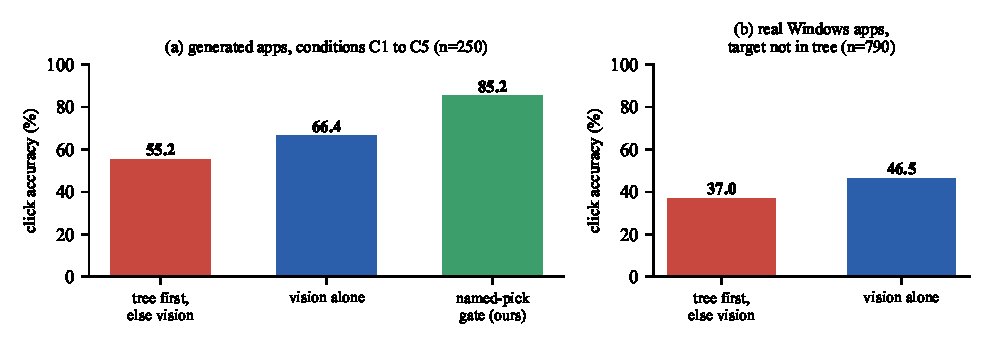
\includegraphics[width=0.92\linewidth]{figures/teaser.pdf}
\caption{\textbf{Trusting the accessibility tree first makes grounding worse than vision alone.}
(a) On generated applications covering five ways a tree can fail (Test A), the common ``tree first, else
vision'' policy loses 11.2 points to our 2B vision grounder on the same 250 items; a gate that trusts the
tree only when an LLM's chosen element has a name gains 18.8. (b) On real Windows applications whose tree
lacks the target (Test B), the tree still answers a quarter of the time and drags accuracy 9.5 points below
vision.}
\label{fig:teaser}
\end{figure}

\section{Introduction}

Every action of a graphical-user-interface (GUI) agent starts with \emph{grounding}: mapping a description
of an element to screen coordinates. Desktop and web platforms expose an \emph{accessibility tree}
(UI Automation on Windows, the DOM accessibility tree in browsers): a list of elements with roles, names
and bounding boxes, built for screen readers. When the tree contains the target and names it, grounding
is a lookup. Trees, however, are often incomplete. Icon buttons ship without names, custom toolkits draw
their own controls, and everything inside a canvas (a spreadsheet grid, a CAD viewport, a whiteboard) is
invisible to them. On the web, 29.6\% of the top million home pages contain at least one button with no
accessible name~\citep{webaim2025}; on the Windows desktop, GIMP's main window exposes seven UI
Automation elements in total (Appendix~\ref{app:exposure}).

Pure-vision grounders~\citep{cheng2024seeclick,lin2025showui,gou2025uground,wu2025osatlas,yang2025ariaui}
avoid the tree entirely, and frontier models now ground from screenshots directly~\citep{anthropic2024computeruse,qin2025uitars}.
Practical systems nevertheless combine the two: UFO2 merges UI Automation controls with a vision
parser~\citep{zhang2025ufo2}, and production browser agents read the accessibility snapshot by default and
request a screenshot only when an element is missing from it~\citep{vardanyan2025browser}. The implicit
policy is \emph{tree first, else vision}.

This policy is safe only if the tree abstains whenever it cannot resolve the target. A name matcher
does not behave that way. Asked for a target that has no name, it returns the element with the closest name;
given two buttons named ``Archive'', it returns the first. In the terms of selective
prediction~\citep{elyaniv2010selective,geifman2017selective}, the tree is a predictor with an abstention
option whose abstention decisions are poorly aligned with its errors. This paper measures the consequences
of that for tree-first agents and proposes a gate that corrects it.

\paragraph{Contributions.}
\begin{enumerate}[leftmargin=*,itemsep=2pt]
\item \textbf{A cheap UIA-supervised grounder} (\S\ref{sec:grounder}). The tree labels its own named
elements for free; 1,572 such examples from ten Windows apps and one free T4 GPU lift Qwen2-VL-2B by
$+44.9$ points on four unseen apps and $+46.1$ on ScreenSpot-v2, including $+57.5$ on phones it never
trained on.
\item \textbf{A controlled per-condition comparison} of tree, vision and hybrid policies with ground truth
from neither source: generated pages in five conditions (Test~A), and real Windows trees damaged on
purpose (Test~B) (\S\ref{sec:compare}).
\item \textbf{The naive merge underperforms vision alone}, with an exact decomposition of why
(Proposition~\ref{prop:decomp}): loss $=$ answer rate $\times$ (tree precision $-$ vision accuracy on the
answered items).
\item \textbf{A gate that works.} Requiring that the LLM's tree pick \emph{has a name} recovers the tree's
strengths without its blindness: 85.2 vs 66.4, and never below vision; the decomposition reproduces its
measured gain (\S\ref{sec:gates}).
\item \textbf{An agent that enforces the gate} (\S\ref{sec:agent}): a loop of perceive, decide, ground, act
and verify in which the LLM only states \emph{what} to act on; a router applies the gate, our grounder supplies
\emph{where}, and task success is read from application state, so false claims of success are counted.
\end{enumerate}
We also list the pipeline failures that would have silently invalidated these results
(Appendix~\ref{app:failures}); several apply to any fine-tuning of a VLM on free hardware.

\section{Related work}

\paragraph{Vision grounders.} SeeClick introduced GUI-grounding pre-training and the ScreenSpot
benchmark~\citep{cheng2024seeclick}. ShowUI~\citep{lin2025showui} shares our base model and trains on
$\sim$256K examples; UGround~\citep{gou2025uground} and Aria-UI~\citep{yang2025ariaui} scale synthetic
web data; OS-Atlas~\citep{wu2025osatlas} synthesises cross-platform data and releases ScreenSpot-v2;
GroundCUA~\citep{feizi2026groundcua} provides 56K human-annotated desktop screenshots; ScreenSpot-Pro~\citep{li2025screenspotpro}
targets high-resolution professional software. Using accessibility metadata to \emph{label} grounding data
is therefore not new; our grounder applies the same idea at a small scale on free hardware, and serves as
the vision side of the comparison.

\paragraph{Hybrid perception in agents.} Set-of-Mark~\citep{yang2023som} and OmniParser~\citep{lu2024omniparser}
turn pixels into candidate elements for a language model; SeeAct~\citep{zheng2024seeact} shows that
grounding, not planning, is the bottleneck of web agents. UFO2~\citep{zhang2025ufo2} fuses UI Automation
with OmniParser detections on Windows, for controls the tree misses. OSWorld~\citep{xie2024osworld} and
Windows Agent Arena~\citep{bonatti2024waa} evaluate agents on real desktop tasks and report grounding as a
main source of failure; ScaleCUA~\citep{liu2025scalecua} scales cross-platform agent data. We found no work
that measures \emph{when the tree's answer should not be trusted}, or that shows a tree-first merge falling
below vision alone.

\paragraph{Uncertainty and abstention.} Selective classification studies predictors that may
abstain~\citep{elyaniv2010selective,geifman2017selective}. For GUI grounding, SafeGround~\citep{wang2026safeground}
calibrates a grounder's own uncertainty from the spread of sampled clicks, and HyperClick~\citep{zhang2025hyperclick}
trains grounders to report calibrated confidence. Both ask when to trust the \emph{grounder}. We ask the
complementary question for the \emph{tree}, and how to arbitrate between the two sources; the two lines
compose (a calibrated grounder could replace our vision branch).

\begin{table}[t]
\centering\small
\begin{tabular}{lccccl}
\toprule
work & reads tree & vision & arbitration measured & per-condition truth & grounder training data \\
\midrule
SeeClick~\citep{cheng2024seeclick} & no & \checkmark & no & no & $\sim$1M examples \\
ShowUI-2B~\citep{lin2025showui} & no & \checkmark & no & no & $\sim$256K examples \\
OS-Atlas~\citep{wu2025osatlas} & labels only & \checkmark & no & no & 13M elements \\
UFO2~\citep{zhang2025ufo2} & \checkmark & \checkmark & no & no & off-the-shelf parser \\
browser agent~\citep{vardanyan2025browser} & \checkmark & on miss & no & no & none \\
SafeGround~\citep{wang2026safeground} & no & \checkmark & grounder only & no & none \\
\textbf{this work} & \checkmark & \checkmark & \checkmark & \checkmark & 1.6K, one free T4 \\
\bottomrule
\end{tabular}
\caption{Positioning. ``Arbitration measured'': when to trust the tree versus vision, per failure condition,
with ground truth from neither source.}
\label{tab:related}
\end{table}

\section{Problem setup}
\label{sec:setup}

A grounding item is a screenshot $s$, an instruction $q$ and a target region $B^\star$. A grounder maps
$(s,q)$ to a point $g \in [0,1000)^2$ in normalised coordinates. The tree $T(s)$ is a set of elements
$e=(\text{role},\text{name},\text{box})$. A tree resolver maps $(T,q)$ to an element or to $\bot$
(abstain); its point is the centre of the element's box. A point \emph{hits} if it lies in $B^\star$;
the same rule scores every method.

\paragraph{Five conditions.} The relation between $q$ and $T$ defines where each source should win:
\textbf{C1 named} (the target is in $T$ under the name $q$ uses), \textbf{C2 unnamed} (in $T$, empty name: an
icon), \textbf{C3 reworded} (in $T$, but $q$ paraphrases its name: ``revert what I just did'' for Undo),
\textbf{C4 canvas} (drawn on a canvas, absent from $T$), \textbf{C5 ambiguous} (several elements share the
target's name; $q$ disambiguates by context, e.g.\ the row it is in; Figure~\ref{fig:c5}).

\paragraph{Policies.} \tree: fuzzy name matching ($\ge$0.6 similarity after dropping action words; ties to
the first element in tree order). \vis: the grounder's point. \fb: \tree{} if it answers, else \vis.
\textsc{snap}: \vis's point moved to the centre of the smallest tree element containing it, or the nearest
within 20 units. \textsc{guarded}: \tree{} only when exactly one element's name equals the instruction's
target words. \textsc{tree\_llm}: an LLM reads $T$ as text and answers one element or NONE.
\textsc{llm\_guarded}: \textsc{tree\_llm}'s pick, else \vis{} on NONE. \textsc{llm\_named}: the pick only
if that element has a non-empty name, else \vis.

\begin{figure}[t]
\centering
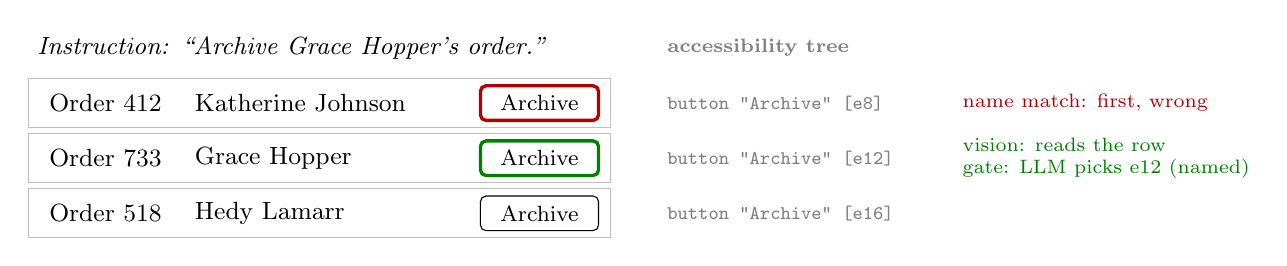
\begin{tikzpicture}[font=\small, row/.style={draw=gray!50, minimum width=7.4cm, minimum height=0.62cm},
  btn/.style={draw, rounded corners=2pt, minimum width=1.5cm, minimum height=0.44cm, font=\footnotesize}]
\node[anchor=west, font=\small\itshape] at (0,2.2) {Instruction: ``Archive Grace Hopper's order.''};
\node[anchor=west, font=\scriptsize\bfseries, gray] at (8.0,2.2) {accessibility tree};
\foreach \y/\o/\p/\r in {1.5/412/Katherine Johnson/e8, 0.8/733/Grace Hopper/e12, 0.1/518/Hedy Lamarr/e16} {
  \node[row, anchor=west] at (0,\y) {};
  \node[anchor=west] at (0.15,\y) {Order \o}; \node[anchor=west] at (2.0,\y) {\p};
  \node[anchor=west, font=\scriptsize\ttfamily, gray] at (8.0,\y) {button "Archive" [\r]};
}
\node[btn, draw=red!70!black, very thick] at (6.5,1.5) {Archive};
\node[btn, draw=green!50!black, very thick] at (6.5,0.8) {Archive};
\node[btn] at (6.5,0.1) {Archive};
\node[anchor=west, font=\scriptsize, red!70!black] at (11.75,1.5) {name match: first, wrong};
\node[anchor=west, font=\scriptsize, green!50!black, align=left] at (11.75,0.8) {vision: reads the row\\gate: LLM picks e12 (named)};
\end{tikzpicture}
\caption{An example of condition C5. The tree lists three identically named buttons; name matching answers
with the first and is wrong, and a tree-first merge never consults vision. An LLM reading the same tree
uses the row text to pick e12; because e12 has a name, the gate trusts it.}
\label{fig:c5}
\end{figure}

\begin{proposition}[Decomposition of a tree-first merge]
\label{prop:decomp}
Let $A$ be the event that the resolver answers ($r \neq \bot$), and $h_r$, $h_g$ the hit indicators of the
tree's and the grounder's points. Then
\begin{align*}
\mathrm{Acc}(\fb) - \mathrm{Acc}(\vis) &= \Pr(A)\,\bigl(\Pr(h_r \mid A) - \Pr(h_g \mid A)\bigr)\\
&= \underbrace{\Pr(A, h_r, \neg h_g)}_{\text{help}} \;-\; \underbrace{\Pr(A, \neg h_r, h_g)}_{\text{harm}} .
\end{align*}
\end{proposition}
\begin{proof}
On $\neg A$ both policies output the grounder's point. On $A$, \fb{} outputs the tree's, so the difference
is $\Pr(A)\,\mathbb{E}[h_r - h_g \mid A]$; expanding $h_r - h_g$ over the four joint outcomes gives the
second form.
\end{proof}

\begin{corollary}
Any policy that uses the tree on a subset $S$ of items and the grounder elsewhere gains
$\Pr(S)\,(\Pr(h_r\mid S)-\Pr(h_g\mid S))$ over \vis. A gate should therefore select the items on which the
tree is \emph{more precise than vision on those same items}; a high precision of the tree in general is
not enough.
\end{corollary}

The identity is elementary. Its use is in what it says to measure: not the tree's overall accuracy, but
its answer rate and its precision on the items it answers, compared with vision's accuracy on those same
items. An incomplete tree causes harm only on items where it still answers.

\section{A UIA-supervised grounder}
\label{sec:grounder}

\subsection{Data}
A declarative registry drives 14 Windows applications through 6 to 10 states each, at 2 or 3 window sizes,
and records the screenshot and the foreground window's UI Automation tree. Each named interactive element
(buttons, menu items, tabs, check boxes, edits, list and tree items, \ldots) becomes a target with an
instruction from a per-control-type template (``Click Save'', ``Open the Find tab''). The result is
200 screenshots and 3,163 targets: train 1,572 and dev 555 from ten apps; \emph{test\_same\_app} 246 (new
screenshots of those apps); \emph{test\_held\_out\_app} 790 from four apps never trained on (Audacity,
Character Map, Device Manager, Notepad++). Geometry variants of one state share its split. Targets are
small: the median box covers 0.11\% of the screen on the held-out apps.

An earlier version of the data passed every schema check but was wrong. Rendering every label onto its
screenshot showed that 36\% of the rows came from the wrong window (focus was lost
mid-collection and the collector walked the code editor's tree), including 100\% of one held-out app. The
collector now verifies the foreground window against the expected application before every state, and a
validation gate rejects wrong-window, out-of-frame and ambiguous rows; privacy guards refuse to collect when
an application restores a previous user session. Appendix~\ref{app:failures} lists these failures.

\subsection{Model and training}
Qwen2-VL-2B-Instruct~\citep{wang2024qwen2vl} with LoRA~\citep{hu2022lora} ($r{=}16$, $\alpha{=}32$,
dropout 0.1) on the language model's attention and MLP projections. The vision tower is frozen and
\emph{run without autograd}: under gradient checkpointing, the library re-enables input gradients on every
sub-model, which put the frozen 32-layer tower into the backward pass. This caused an out-of-memory error on the
T4; earlier runs that fit averaged about 57\,s per step, against 20.8\,s after the fix. Training uses fp16 on a Kaggle T4 with the adapter
held in fp32 and loss scaling, learning rate $10^{-4}$, 3\% warm-up, effective batch 4, three epochs
(1,179 steps, 8.0\,h, 8.5\,GB peak). The model answers a point \texttt{(x,y)} in $[0,1000)$ coordinates.

\subsection{Evaluation protocol}
Hypotheses H1 to H6 were committed before the data they concern existed. The checkpoint was chosen by click
accuracy on a seeded 200-example dev subset among all saved steps, and the choice was pushed before any
test example was scored; each test set was scored once, with greedy decoding. The parser is deliberately
generous to the zero-shot baseline, which answers in its pre-training box format on 517 of 1,591 items:
boxes in any of three syntaxes are scored at their centre. Intervals are paired bootstrap 95\% CIs,
resampled by \emph{screenshot}, since targets on one screen are correlated.

\section{Grounder results}

\begin{table}[t]
\centering\small
\begin{tabular}{lccc}
\toprule
& zero-shot & fine-tuned & $\Delta$ [95\% CI, screenshot-clustered] \\
\midrule
test\_same\_app ($n{=}246$) & 14.2 & 64.6 & $+50.4$ [43.0, 57.8] \\
test\_held\_out\_app ($n{=}790$) & 1.5 & \textbf{46.5} & $+44.9$ [41.1, 48.7] \\
ScreenSpot-v2, 6-cell mean ($n{=}1{,}272$) & 19.2 & 62.8 & $+46.1$ [42.9, 49.1] \\
\bottomrule
\end{tabular}
\caption{Click accuracy (\%). H1 (same apps) and H3 (unseen apps) are supported; the gain holds on each
unseen app: Audacity 3.1$\to$48.0, Character Map 1.7$\to$52.1, Device Manager 0.0$\to$37.2, Notepad++
1.6$\to$51.0.}
\label{tab:grounder}
\end{table}

\begin{figure}[t]
\centering
\begin{subfigure}{0.49\linewidth}\centering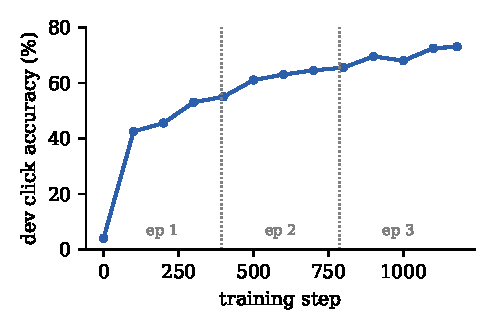
\includegraphics[width=\linewidth]{figures/learning_curve.pdf}
\caption{Dev accuracy by step (zero-shot = step 0).}\end{subfigure}
\begin{subfigure}{0.49\linewidth}\centering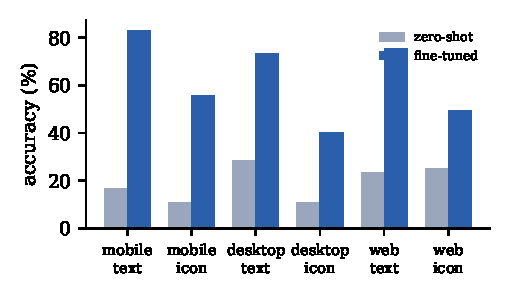
\includegraphics[width=\linewidth]{figures/screenspot_v2.pdf}
\caption{ScreenSpot-v2 by platform and target type.}\end{subfigure}
\caption{The grounder is still improving at the last step (4.0$\to$73.0\% on dev), and the gain transfers
to every ScreenSpot-v2 platform, phones most ($+57.5$), though it trained only on Windows.}
\label{fig:grounder}
\end{figure}

Table~\ref{tab:grounder} and Figure~\ref{fig:grounder} summarise the grounder. On ScreenSpot-v2 every cell
improves: mobile text 16.6$\to$83.1 and icons 10.9$\to$55.9; desktop text 28.4$\to$73.2 and icons
10.7$\to$40.0; web text 23.5$\to$75.2 and icons 25.1$\to$49.3. Text targets beat icons on every platform.
On the original ScreenSpot our 6-cell mean is 61.9, between SeeClick's 53.4 (9.6B parameters,
$\sim$1M examples) and ShowUI-2B's 75.1 (same base model, $\sim$256K examples); cross-paper numbers differ in
prompts and resolution and are for orientation only.

\paragraph{How it misses.} Target size dominates (Figure~\ref{fig:size}): on unseen apps hit rate is 15.2\%
for the smallest quartile of boxes and about 65\% for the two largest. By control type, menu items
(65.0\%, $n{=}240$) and combo boxes (69.0\%) are easy; buttons (36.0\%, $n{=}278$), tree items (29.1\%) and
edits (21.1\%) are hard. Half the misses on unseen apps land within 50 units of the right box (18.7\%
within 10 units, 33.3\% between 10 and 50): the model found the right region but chose a neighbouring
element. On ScreenSpot two thirds of the misses are farther than 50 units, which indicates that the
instruction itself was not understood.

\begin{figure}[t]
\centering
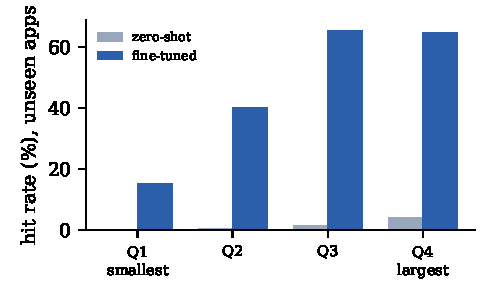
\includegraphics[width=0.48\linewidth]{figures/size_quartiles.pdf}
\caption{Hit rate on unseen apps by quartile of target area (median areas 540 to 4,050 units$^2$ of
$10^6$). The grounder is weakest on small targets such as toolbar icons and tree-view arrows.}
\label{fig:size}
\end{figure}

\section{Tree, vision, or both}
\label{sec:compare}

\subsection{Test A: generated pages}
We generate web pages in which every target's true box comes from the DOM or the canvas geometry, so that
neither method grades itself. Each page carries one target per condition; the condition is verified on the
rendered tree and pixels. Dev pages (seeds 0 to 11 and 100 to 159) were used to design rules; the frozen test set is
seeds 1000 to 1199: 1,000 items, 200 per condition.

\begin{table}[t]
\centering\small
\begin{tabular}{lcccccc}
\toprule
policy & C1 named & C2 unnamed & C3 reworded & C4 canvas & C5 ambiguous & mean \\
\midrule
\tree{} (name match) & \textbf{100.0} & 0.0 & 0.0 & 0.0 & 26.5 & 25.3 \\
\vis, zero-shot & 60.5 & 7.5 & 0.0 & 47.5 & 40.5 & 31.2 \\
\vis, fine-tuned & 94.0 & 40.0 & 31.0 & \textbf{99.0} & 65.0 & 65.8 \\
\fb{} (tree, else vision) & 100.0 & 37.5 & 29.5 & 75.5 & 26.5 & 53.8 \\
\textsc{snap} & 94.5 & 41.0 & 33.0 & 99.0 & 70.5 & 67.6 \\
\textsc{guarded} & 100.0 & 40.0 & 31.0 & 99.0 & 65.0 & 67.0 \\
\bottomrule
\end{tabular}
\caption{Test A, click accuracy (\%), 200 items per condition. The tree wins only C1 (H4: $+6.0$
[3.0, 9.5]); vision wins unnamed icons ($+40.0$) and canvas ($+99.0$) (H5). \fb{} loses $12.0$ points
[9.7, 14.4] to vision alone (page-clustered).}
\label{tab:testa}
\end{table}

\begin{table}[t]
\centering\small
\begin{tabular}{lcccccc}
\toprule
& C1 & C2 & C3 & C4 & C5 & all \\
\midrule
tree answers, $\Pr(A)$ & 100.0 & 4.5 & 6.0 & 23.5 & 100.0 & 46.8 \\
tree precision when answering & 100.0 & 0.0 & 0.0 & 0.0 & 26.5 & 54.1 \\
vision accuracy on those items & 94.0 & 55.6 & 25.0 & 100.0 & 65.0 & 79.7 \\
\midrule
help: tree right, vision wrong & 6.0 & 0.0 & 0.0 & 0.0 & 11.0 & 3.4 \\
harm: tree wrong, vision right & 0.0 & 2.5 & 1.5 & 23.5 & 49.5 & 15.4 \\
\fb{} $-$ \vis{} & $+6.0$ & $-2.5$ & $-1.5$ & $-23.5$ & $-38.5$ & $-12.0$ \\
\bottomrule
\end{tabular}
\caption{Proposition~\ref{prop:decomp} on Test A (\% of items). The tree abstains on most unnamed and
reworded targets, but answers every ambiguous item and a quarter of canvas items (where another page
element has a similar name). Over all items it answers, it is right 54\% of the time, against 80\% for
vision on the same items.}
\label{tab:decomp}
\end{table}

Table~\ref{tab:testa} shows the comparison and Table~\ref{tab:decomp} its decomposition. The loss of the
naive merge comes from items where the tree answers and is wrong: on C5 it answers every item, picks the
first of the same-named buttons, and overrides a correct vision click on 49.5\% of items; on C4 a similarly
named element elsewhere on the page overrides vision on 23.5\%. Where the tree abstains (C2, C3) the merge
costs little. \textsc{snap} is the best rule without an LLM ($+1.8$ [1.1, 2.6] over vision),
and \textsc{guarded} fixes the grounder's C1 slips and otherwise equals it.

\begin{figure}[t]
\centering
\begin{subfigure}{0.49\linewidth}\centering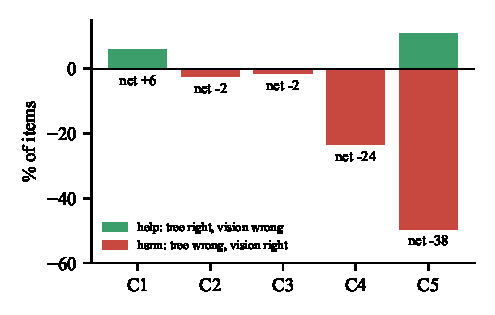
\includegraphics[width=\linewidth]{figures/test_a_help_harm.pdf}
\caption{Test A: help and harm of \fb{} per condition.}\end{subfigure}
\begin{subfigure}{0.49\linewidth}\centering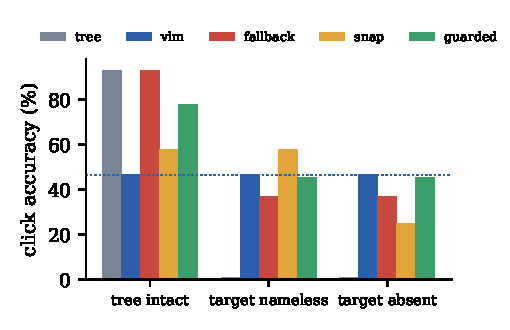
\includegraphics[width=\linewidth]{figures/test_b.pdf}
\caption{Test B: unseen apps, three tree states.}\end{subfigure}
\caption{(a) The merge loses because of harm (tree wrong, vision right), not because of missing help. (b) On real screens, \vis{} (dotted) is unaffected by
the tree; \fb{} and \textsc{snap} fall below it once the target is missing, \textsc{guarded} does not.}
\label{fig:merge}
\end{figure}

\subsection{Test B: real Windows trees, damaged on purpose}
The grounder never reads the tree, so its saved answers on the real test screenshots can be re-scored
against the real UI Automation tree in three states: \emph{intact}; \emph{nameless} (the target's name
blanked, a real-screen C2); and \emph{absent} (the target removed, a real-screen C4). The stored tree holds
the named elements of each screenshot, so it is cleaner than a live one; the results are therefore
favourable to the tree.

\begin{table}[t]
\centering\small
\begin{tabular}{llccccc}
\toprule
split & tree state & \tree & \vis & \fb & \textsc{snap} & \textsc{guarded} \\
\midrule
\multirow{3}{*}{unseen apps ($n{=}790$)} & intact & 92.8 & 46.5 & 93.0 & 58.0 & 77.8 \\
& nameless & 1.0 & 46.5 & 37.0 & 58.0 & 45.3 \\
& absent & 1.0 & 46.5 & 37.0 & 24.8 & 45.3 \\
\midrule
\multirow{3}{*}{same apps ($n{=}246$)} & intact & 85.0 & 64.6 & 85.0 & 67.9 & 85.0 \\
& nameless & 0.4 & 64.6 & 46.3 & 67.9 & 63.8 \\
& absent & 0.4 & 64.6 & 46.3 & 47.6 & 63.8 \\
\bottomrule
\end{tabular}
\caption{Test B, click accuracy (\%). Screenshot-clustered differences against \vis{} on unseen apps:
\fb{} with a blind tree $-9.5$ [$-11.8$, $-7.4$]; \textsc{snap} $+11.5$ [9.4, 13.9] intact and $-21.6$
[$-25.6$, $-17.8$] absent; \textsc{guarded} $+31.4$ [27.1, 35.9] intact and $-1.1$ [$-1.9$, $-0.5$] blind.}
\label{tab:testb}
\end{table}

The same failure appears on real screens (Table~\ref{tab:testb}). With the target missing, the tree still
answers on 25.8\% of unseen-app items, because another element shares or resembles the target's name, and
it is right on 3.9\% of those, against 40.7\% for vision: $0.258 \times (3.9 - 40.7) = -9.5$. On the same
apps the loss is $-18.3$. Even an intact tree is imperfect for name matching: 23.2\% of same-app targets
share their exact name with another element on screen (the real-world C5), and with the intact same-app
tree \fb{} helps on 28.9\% of items but harms on 8.5\%. Snapping vision onto the tree helps when the target
is in the tree, named or not, and costs 21.6 points when it is not. A good hybrid therefore needs to know
whether the tree contains the target, which is the signal the gates below provide.

\subsection{Gates: letting the tree say ``I don't know''}
\label{sec:gates}

\begin{table}[t]
\centering\small
\begin{tabular}{lcccccc}
\toprule
policy & C1 & C2 & C3 & C4 & C5 & mean \\
\midrule
\tree{} (name match) & 100 & 0 & 0 & 0 & 32 & 26.4 \\
\fb{} & & & & & & 55.2 \\
\vis & 98 & 38 & 28 & 100 & 68 & 66.4 \\
\textsc{guarded} & 100 & 38 & 28 & 100 & 68 & 66.8 \\
\textsc{tree\_llm} & 88 & 2 & 88 & 0 & 100 & 55.6 \\
\textsc{llm\_guarded} (pre-registered) & 92 & 32 & 92 & 100 & 100 & 83.2 \\
\textbf{\textsc{llm\_named}} (chosen on dev) & 94 & 38 & 94 & 100 & 100 & \textbf{85.2} \\
\bottomrule
\end{tabular}
\caption{The 250-item LLM subset of Test A (first 50 test pages, fixed in advance), all policies on the
same items. \textsc{llm\_named} $-$ \vis{} $+18.8$ [15.2, 22.4]; $-$ \textsc{llm\_guarded} $+2.0$
[0.4, 4.0] (pages resampled). The LLM (gpt-oss-120b, temperature 0) used 555 tokens per item.}
\label{tab:gates}
\end{table}

An LLM reading the tree (\textsc{tree\_llm}) removes the tree's wording and ambiguity problems (C3 88, C5
100) but not its blindness (C2 2, C4 0). We pre-registered \textsc{llm\_guarded}: the LLM's NONE hands the
item to vision. It reached 83.2, but lost 6 points to vision on unnamed icons: on 15 of the 50, the LLM picked an
element instead of answering NONE, 8 of them nameless. Four candidate repairs and a selection rule were then
frozen before any dev answer existed; on 300 new dev items \textsc{llm\_named} tied for best (84.3) and,
being simplest, was chosen; it was scored once on the test subset (Table~\ref{tab:gates}). It is never below
vision on any condition.

\begin{table}[t]
\centering\small
\begin{tabular}{lccc}
\toprule
LLM answer & share of items & LLM precision & vision accuracy on these items \\
\midrule
a named element & 59.2 & \textbf{93.2} & 61.5 \\
a nameless element & 4.0 & 10.0 & 60.0 \\
NONE & 36.8 & n/a & 75.0 \\
\bottomrule
\end{tabular}
\caption{Why a name is the right abstention signal (250 items, \%). A named pick is far more precise than
vision on the same items; a nameless pick is far less. By the corollary of Proposition~\ref{prop:decomp},
\textsc{llm\_named} should gain $0.592 \times (93.2 - 61.5) = +18.8$ points over vision, and
\textsc{llm\_guarded} $0.632 \times (87.9 - 61.4) = +16.8$: both are the measured differences.}
\label{tab:audit}
\end{table}

Table~\ref{tab:audit} explains the result. The LLM's named picks are 93.2\% precise where vision is 61.5\%
on the same items; its nameless picks are 10\% precise where vision is 60\%. Requiring a name selects
the subset on which the tree's pick beats vision, which is the condition the corollary sets for a gate. The remaining
errors are C1 slips on one-word instructions (``Translate'' answered with Sort) and, on dev only, two canvas
targets for which the LLM named a similarly named page element.

\section{Enforcing the gate in an agent}
\label{sec:agent}

\begin{figure}[t]
\centering
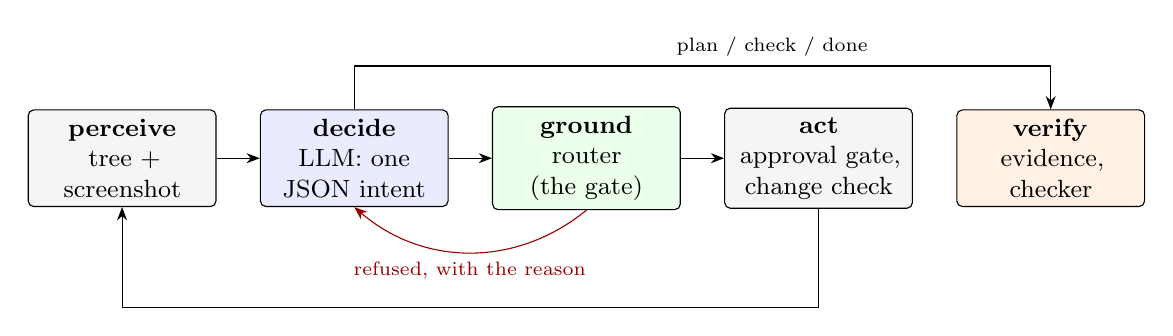
\begin{tikzpicture}[node distance=0.55cm and 0.55cm, box/.style={draw, rounded corners=2pt, align=center,
  font=\small, minimum height=1.05cm, text width=2.15cm, fill=#1}, box/.default=white, >=Stealth]
\node[box=gray!8] (p) {\textbf{perceive}\\ tree + screenshot};
\node[box=blue!8, right=of p] (d) {\textbf{decide}\\ LLM: one JSON intent};
\node[box=green!8, right=of d] (g) {\textbf{ground}\\ router (the gate)};
\node[box=gray!8, right=of g] (a) {\textbf{act}\\ approval gate, change check};
\node[box=orange!10, right=of a] (v) {\textbf{verify}\\ evidence, checker};
\draw[->] (p) -- (d); \draw[->] (d) -- (g); \draw[->] (g) -- (a);
\draw[->] (a.south) -- ++(0,-1.25) -| (p.south);
\draw[->] (d.north) -- ++(0,0.55) -| node[pos=0.3, above, font=\scriptsize]{plan / check / done} (v.north);
\draw[->, red!60!black] (g.south) to[bend left=40] node[below, font=\scriptsize]{refused, with the reason} (d.south);
\end{tikzpicture}
\caption{The loop (LangGraph). Only \emph{decide} is a language model; it states what to act on. The router
places it: a named tree element through the tree, a description through our grounder, a nameless id or bare
coordinates are refused with a reason. Success is read from the application, not from the LLM.}
\label{fig:loop}
\end{figure}

In an agent the decision-making LLM already reads the tree, so it can play the role of the gate's LLM at no
extra cost. Figure~\ref{fig:loop} shows the loop. Each turn the LLM returns one intent, for example
\begin{center}\small
\verb|{"action": "click", "target": "the floppy-disk save icon"}|\quad or\quad
\verb|{"action": "type", "element": "e27", "text": "..."}|
\end{center}
The router enforces \textsc{llm\_named}: an element id is accepted only if that element is named; a
description is sent to the grounder; bare click coordinates are refused (drawing on an empty canvas, where
there is nothing to ground, is the one exception, and is labelled as such). Every action records which
channel placed it (tree, grounder, or the LLM's own reading). The approval gate for consequential actions
(send, delete, purchase) inspects the element \emph{under} the point, so coordinates cannot bypass it.
``Done'' is a claim: plan steps must be checked with evidence the system verifies (text on screen, a fresh
file, a changed screen, a URL), and a task-specific checker reads the application's state; a claim the
checker rejects is a \emph{false success}.

\paragraph{Sandbox suite.} Five web tasks, one per condition, regenerated per seed, each with a checker
that reads application state: a sign-up form whose labels differ from the goal's words (C1/C3); a notes
app whose only working save control is a nameless icon (C2); a mixer whose buttons are drawn on a canvas
(C4); three rows with identically named ``Archive'' buttons (C5); and drawing a line between two dots
(drag). Four arms vary what the brain sees and who places clicks: A, the LLM on screenshots placing its
own clicks; B, the LLM on the tree only; C, the LLM with tree and screenshot behind the router and our
grounder; D, a free text-only LLM behind the router and our grounder.

\paragraph{Serving the grounder.} On the development laptop the grounder fits in memory only with 8-bit
dynamic quantisation of every linear layer, and quantised it hit 1 of 12 held-out targets, answering in the
base model's formats (\texttt{<ref>Window 1</ref>}) rather than points: naive quantisation of the vision
tower and adapter erased the fine-tuning. We therefore serve the unmodified model from a free T4 over an
authenticated tunnel; on 40 held-out examples its answers are identical, coordinate for coordinate, to the
stored evaluation predictions (65\% on that sample), at a median of 4.7\,s per call round trip.

\pending{Task-level results for arms A to D over 5 tasks $\times$ 3 seeds: pass rate with CI, pass-all-seeds,
false-success rate, actions, tokens, channel mix.}

\paragraph{Case study.} On Excalidraw, the toolbar is fully named in the accessibility tree, while shapes
drawn on the board are absent from it: after drawing two labelled boxes and an arrow, neither label appears
in the snapshot. A checker reading the application's autosave confirms labels and that arrows are bound to
both shapes. Tool selection is a tree action; anything referring to existing drawings must go through the
grounder. \pending{demo episode and its channel trace.}

\section{Discussion and limitations}

\paragraph{Abstention, not merging.} The tree is exact when it has the target, and it does not report
when it lacks it. The results point to a better abstention signal rather than a better merge rule, and
Proposition~\ref{prop:decomp} states the criterion: a gate should hand an item to the tree when the tree
is more precise than vision \emph{on that item}. Whether the selected element has a name is a cheap proxy
for that criterion, and in our data a strong one. The argument is not specific to UI
Automation; it applies to any structured source an agent might trust first: DOM selectors, OCR, or an API
index.

\paragraph{Limitations.}
\begin{itemize}[leftmargin=*,itemsep=1pt]
\item One training seed \pending{second seed's evaluation (trained)}; four unseen apps, so app-level
intervals are wide (\textsc{guarded} intact: [20.9, 41.6] resampling apps).
\item \textbf{The teacher labels only what it names.} Every training target is a named element, yet the
grounder's role in the gate is the nameless and the absent; unnamed icons remain vision's weakest condition
(38 to 40\%). \pending{Test C: real targets the tree cannot see, $\sim$250 hand-drawn boxes across 8 apps.}
\item Test A is synthetic; Test B's stored tree is cleaner than a live one; the LLM gate was confirmed on
250 synthetic items and costs one LLM call per grounding outside an agent.
\item Instructions are templated from names; reworded instructions (C3) score 31 for vision alone.
\item Element-level results; task-level results are pending (\S\ref{sec:agent}).
\end{itemize}

\section{Conclusion}
Asking the accessibility tree first is a common design for computer-use agents. When the tree is
incomplete, it lowers grounding accuracy below that of vision alone, because the tree keeps answering on
items it cannot resolve and its errors override a more accurate vision model. The tree's answer rate and
its precision on the items it answers account for the loss exactly. A gate that trusts only named tree
picks keeps the tree's advantage on named targets without the loss, and a 2B grounder trained on the tree's
own labels on free hardware is accurate enough to serve as the vision side.

\paragraph{Reproducibility.} Code, notebooks pinned to commits, the sandbox generator, the per-example
results and \texttt{scripts/paper\_numbers.py} (which regenerates every number and figure here) are at
\url{https://github.com/rudranaresh0201/computer-use}. The dataset is not released pending a privacy audit.

\bibliographystyle{plainnat}
\bibliography{refs}

\appendix

\section{Training and evaluation details}
\begin{table}[H]
\centering\small
\begin{tabular}{ll}
\toprule
base model & Qwen2-VL-2B-Instruct; vision tower frozen, run under \texttt{no\_grad} \\
adapter & LoRA $r{=}16$, $\alpha{=}32$, dropout 0.1, attention and MLP projections of the language model \\
optimisation & AdamW, lr $10^{-4}$, linear decay, 3\% warm-up, effective batch 4, 3 epochs = 1,179 steps \\
precision & fp16 base, fp32 adapter, loss scaling (T4: no bf16 tensor cores) \\
hardware & one Kaggle T4 (16\,GB): 20.8\,s/step, 8.5\,GB peak, 8.0\,h, checkpoints pushed to the Hub \\
output & \texttt{(x,y)} in $[0,1000)$; greedy decoding, 48 new tokens \\
selection & click accuracy on a seeded 200-item dev subset over all snapshots; step 1179 chosen \\
images & 1568$\times$882 (training pixel budget); ScreenSpot images scaled down only, aspect kept \\
\bottomrule
\end{tabular}
\end{table}

\section{Pipeline failures that would have invalidated results}
\label{app:failures}
Each of these passed tests and produced plausible numbers.
\begin{table}[H]
\centering\small
\begin{tabular}{p{4.2cm}p{5.2cm}p{4.6cm}}
\toprule
failure & symptom & how found / fixed \\
\midrule
labels from the wrong window & 36\% of rows (100\% of one held-out app) described another application & rendering labels onto images; foreground verification per state \\
first-$N$ sampling per control type & tree order visits window chrome first: data collapsed to Minimize/Close & audit; random sampling within the cap \\
fp16 without loss scaling & adapter updates underflowed to zero; sane loss, unstable runs & audit; fp32 adapter + GradScaler \\
frozen tower in backward pass & OOM; $\sim$3$\times$ slower steps & memory arithmetic of the OOM; tower under \texttt{no\_grad} \\
emulated bf16 on a T4 & math attention kernel, full attention matrix & checking compute capability, not \texttt{is\_bf16\_supported} \\
per-chunk LR schedule & LR would decay to zero at each chunk's end & reading the notebook before running \\
box answers scored at a corner & zero-shot penalised for syntax, inflating H1 & eval smoke; boxes scored at centre in all syntaxes \\
session restore on cold launch & a previous user's file tab entered the data & label review; refuse unexpected tabs \\
\bottomrule
\end{tabular}
\end{table}

\section{Pre-registration and freezes}
Hypotheses H1 to H6 and every rule were committed before the data they concern: training code
\texttt{d1e135a}; evaluation \texttt{ad1446a}; \textsc{guarded} \texttt{d665c19}; \textsc{tree\_llm}
\texttt{938f46a}; \textsc{llm\_guarded} \texttt{1ad9836}; gate candidates and selection rule
\texttt{1cc4d26}; final GPU run \texttt{c089d74}.

\section{The tree prompt}
\begin{small}
\begin{verbatim}
You see the accessibility tree of an application window, the way a screen reader
sees it: one element per line as  role "name" [ref=...], indented by nesting.
Headings and regions give context. Buttons with no name have no text in the tree.

Instruction: {instruction}

Which ONE element should be clicked to follow the instruction? Answer with only its
ref (for example e12). If no element in the tree can be identified as the target,
answer NONE.

Tree:
{tree}
\end{verbatim}
\end{small}
Model \texttt{openai/gpt-oss-120b} (Groq), temperature 0, reasoning effort low. The tree keeps interactive
elements, headings and landmark regions, without boxes.

\section{What UI Automation exposes on eight real applications}
\label{app:exposure}
\begin{table}[H]
\centering\small
\begin{tabular}{lrrr}
\toprule
application (main window) & UIA elements & named interactive & nameless interactive \\
\midrule
GIMP & 7 & 4 & 0 \\
VLC & 36 & 12 & 11 \\
Excalidraw (in Chrome) & 44 & 17 & 0 \\
Git GUI & 62 & 12 & 0 \\
Notepad++ & 68 & 21 & 32 \\
Audacity & 151 & 56 & 2 \\
VS Code & 162 & 71 & 0 \\
Paint & 173 & 111 & 1 \\
\bottomrule
\end{tabular}
\caption{One capture per application. Counts describe what the tree exposes, not what a person can click;
measuring the latter needs hand-drawn labels \pending{Test C/D}.}
\end{table}

\end{document}
